% ============================================================
% MCM/ICM style paper
% Multi-Vehicle Cooperative Rapid Geolocation of UAV Alerts
% Compile: pdflatex -> pdflatex  (no bibtex needed, manual bibliography)
% ============================================================
\documentclass[12pt]{article}

\usepackage{fontspec}
\setmainfont{Times New Roman}
\setsansfont{Arial}
\usepackage[margin=1in]{geometry}
\usepackage{graphicx}
\graphicspath{{figures/}{../figures/}}
\usepackage{amsmath,amssymb,bm}
\usepackage{booktabs}
\usepackage{multirow}
\usepackage{caption}
\usepackage{subcaption}
\usepackage{enumitem}
\usepackage{listings}
\usepackage{xcolor}
\usepackage{array}
\usepackage[hidelinks]{hyperref}

\lstset{basicstyle=\ttfamily\scriptsize,frame=single,numbers=left,numbersep=6pt,
  breaklines=true,columns=fullflexible,keepspaces=true,showstringspaces=false,
  language=Python,commentstyle=\color{green!45!black},keywordstyle=\color{blue!70!black},
  stringstyle=\color{red!55!black}}

\captionsetup{font=small,labelsep=period}
\setlist{itemsep=2pt,topsep=3pt,parsep=0pt}

\newcommand{\paperfig}[4][0.9]{%
  \begin{figure}[htbp]
    \centering
    \includegraphics[width=#1\textwidth]{#2}%
    \caption{#3}\label{#4}
  \end{figure}}

\title{\bfseries Multi-Vehicle Cooperative Rapid Geolocation of UAV Alerts:\\[3pt]
\large Analytical Observability, an Intersection-Accuracy Lower Bound,\\
and Disruption-Aware Rescheduling}
\author{}
\date{}

\begin{document}

\begin{center}
{\LARGE\bfseries Multi-Vehicle Cooperative Rapid Geolocation of UAV Alerts}\\[6pt]
{\large Analytical Observability, an Intersection-Accuracy Lower Bound,\\[2pt]
and Disruption-Aware Rescheduling}
\end{center}

\vspace{6pt}
\begin{center}{\large\bfseries Summary}\end{center}

\begingroup
\small
\setlength{\parskip}{3pt}

Small unmanned aerial vehicles (UAVs) that violate airspace rules must be located within seconds. A practical and low-cost architecture uses a handful of ground vehicles carrying pan--tilt--zoom cameras: each vehicle drives to a vantage point, points its gimbal upward at a steep elevation, and two or more azimuth measurements are intersected to recover the target's three-dimensional position. The design question is therefore twofold and coupled: \emph{where should each camera stand}, and \emph{who should go where, when}. We build a three-layer model---geometry, measurement, decision---shared by all five sub-problems, so that occlusion, drivable space, gimbal kinematics, and the observation timeline are defined exactly once. The shared layer is validated by five independent cross-checks (20\,000-point drivable-space test, 1\,800-sample line-of-sight test, zero-wall-crossing path audit, five hand-computed gimbal cases, and a hand-computed timeline), all of which pass.

\textbf{For Problem 1} we minimize the horizontal standoff $r$. The elevation cap yields a provable lower bound $r\ge r_{\mathrm{lb}}=(H-2)/\tan 80^\circ=7.58206$ m; because a feasible point exists on that circle, a two-dimensional search collapses to a \emph{one-dimensional arc enumeration}. A 0.2 m grid (251\,000 points) gives an observable area of $5\,607.8\ \mathrm{m^2}$, of which 63\,435 points are removed by occlusion alone (30.6\% of the drivable area)---occlusion, not geometry, is the binding constraint. The optimal set is a single $283.85^\circ$ arc; a three-level tie-break (maximum clearance, then minimum distance to the depot, then minimum bearing) selects $(88.8247,\,76.3233)$ with $r=7.5821$ m, elevation $80.0^\circ$, and $Q=1/r=0.131890\ \mathrm{m^{-1}}$, within 0.04 mm of the analytical bound.

\textbf{For Problem 2(1)} first-order propagation gives $\sigma_p=\sigma\sqrt{r_1^2+r_2^2}/|\sin\gamma|$, whose global minimum $\sigma\sqrt2\,r_{\mathrm{lb}}=0.14362$ m is attained simultaneously at $r_1=r_2=r_{\mathrm{lb}}$ and $\gamma=90^\circ$. A 0.5 m exhaustive grid plus 0.02 m refinement selects vehicles V3--V5 with stations $(5.3448,73.7448)$ and $(12.2737,78.1841)$, baseline $8.229$ m, giving $\sigma_p=0.14362$ m (95\% circle $0.2486$ m). A 200\,000-sample Monte Carlo reproduces the RMS to $0.01\%$.

\textbf{For Problem 2(2)} we enumerate all 360 reuse structures and evaluate each with a fixed-point timeline. The optimum is $t_{\mathrm{last}}=10.655$ s (T1 $2.678$, T2 $10.255$, T3 $10.655$ s). The structural reason is decisive: V3 serves T1 and then T3 \emph{from the same station} $(13.5,91.0)$, so the reuse costs no repositioning at all. This is $45.9\%$ faster than a nearest-assignment heuristic ($19.691$ s) and matches a hand-computed chain to 1 ms.

\textbf{For Problem 3} the composite pointing error $\sigma_{\Delta\psi}=\sqrt{\arctan^2(\sigma(s)/r)+0.8^2+0.6^2}$ inverts to a maximum travel $s_{\max}=66.968$ m. At $80$ m the requirement becomes $a+80b\le1.6394$ m, which the nominal $(0.3,0.02)$ pair violates ($1.90$ m, pass rate $0.9156$). Two million Monte Carlo samples agree with the closed form to $0.0069^\circ$, and Kolmogorov--Smirnov tests ($p=0.92$, $0.67$) do not reject normality.

\textbf{For Problem 4} we compare keeping the original plan against online rescheduling on 93 disruption scenarios. Rescheduling wins 88, ties 5, and loses \emph{none}; mean alert completeness rises from $0.8566$ to $1.0000$ and mean $t_{\mathrm{last}}$ falls from $23.99$ to $22.37$ s. The gains decompose cleanly: new-alert cases buy \emph{time} ($-5.23$ s), vehicle-failure and combined cases buy \emph{completeness} ($\eta$ $+0.27$), and communication cases are correctly left untouched.

Our contributions are (i) replacing a 2-D search by an analytical bound that makes the single-station optimum \emph{provable} and the tie-break reproducible; (ii) identifying same-station reuse, which converts scheduling from continuous-time optimization into a 360-case structural search; and (iii) a fallback rule that makes ``never worse than the original plan'' a structural guarantee rather than an empirical hope.

\vspace{4pt}
{\footnotesize\noindent\textbf{Keywords:} UAV geolocation; bearings-only intersection; observable region; visibility graph; vehicle scheduling; disruption rescheduling}
\endgroup

\newpage
\setcounter{page}{2}

% ============================================================
\section{Introduction}

\subsection{Background and Problem Restatement}

A $100\ \mathrm{m}\times100\ \mathrm{m}$ urban block (origin at the south-west corner, $x$ east, $y$ north) contains five axis-aligned box buildings B1--B5 and five ground vehicles V1--V5. A UAV alert is reported as a bearing $\theta$, a horizontal range $R$, and an altitude $H$ measured from the block centre, so that the target sits at
\begin{equation}
\label{eq:target}
(x_T,y_T)=(50+R\cos\theta,\ 50+R\sin\theta),\qquad z_T=H .
\end{equation}
Three alerts are given: T1 $=(30^\circ,40,45)$, T2 $=(150^\circ,45,35)$, T3 $=(285^\circ,38,55)$, i.e.\ targets at $(84.6410,70.0000)$, $(11.0289,72.5000)$ and $(59.8351,13.2948)$ with altitudes $45$, $35$ and $55$ m.

A vehicle is a disc of radius $1.5$ m that must keep at least $1.5$ m clearance from every building; its centre is the station. It drives at $3$ m/s. The camera sits $2$ m above ground; the gimbal covers elevation $[-10^\circ,80^\circ]$ and slews at $30^\circ/\mathrm{s}$ on both axes simultaneously, the slower axis determining the duration. A joint observation lasts $5$ s. While driving, the gimbal stays level and pointing east.

Buildings are impenetrable to line of sight. The five tasks are: (1) characterise the observable region for T1 and pick the best single station; (2) build a two-station intersection error model and select the best pair of vehicles and stations for T2; (3) schedule all three concurrent alerts with five vehicles, allowing one vehicle to serve two alerts, minimising the last observation start; (4) determine how far a vehicle may drive before pointing accuracy degrades below a $95\%$ requirement; and (5) design and evaluate a rescheduling policy under disruptions.

\subsection{Why the Sub-Problems Form One Chain}

The five tasks are not independent. Problem 1 characterises \emph{single-station} feasibility. Problem 2(1) layers a \emph{two-station} accuracy metric on top of it. Problem 2(2) downgrades accuracy to a feasibility predicate and optimises \emph{time}. Problem 3 quantifies how much time may be spent before accuracy is lost. Problem 4 tests the resulting plan under \emph{perturbation}. Consequently we do not write a separate geometry engine per sub-problem: we build one scene layer---drivable space, occlusion test, gimbal kinematics, timeline---and call it from everywhere. The benefit is single-source-of-truth semantics: if the boundary convention of the occlusion test were changed in one place, the other four sub-problems would immediately become inconsistent and the cross-checks would fail.

\subsection{Our Approach in One Paragraph}

Geometry: convert ``can we see it'' into a segment--closed-box intersection and ``can we stand here'' into a point--rectangle distance, both analytic and vectorisable. Measurement: convert ``how accurate'' into the trace of a first-order covariance, and ``how soon'' into a shortest-path plus gimbal-slew time chain. Decision: solve a constrained minimisation (Problem 1), a minimax continuous programme (Problem 2(1)), and a discrete structural search (Problems 2(2) and 4). Every sub-problem keeps at least two independent solution paths, and at least one of them does not rely on optimisation search---a closed-form bound, a Monte Carlo estimate, or a hand-computed chain---precisely so that we can tell whether the optimiser actually converged.

% ============================================================
\section{Assumptions and Notation}

\subsection{Assumptions}

\begin{enumerate}[leftmargin=2em]
  \item \textbf{Buildings are opaque closed boxes}; a sight line touching an edge, a face or a vertex counts as blocked. \emph{Rationale:} at grazing incidence the image is unusable for bearing measurement, and the closed convention is the conservative one. Used in \eqref{eq:block}.
  \item \textbf{Vehicles are discs of radius 1.5 m with instantaneous turning and no acceleration limit}, travelling at a constant $3$ m/s. \emph{Rationale:} the problem states no acceleration bound; at $3$ m/s the ramp-up lasts well under a second, negligible against a $10$ s timeline. Used in \eqref{eq:travel}.
  \item \textbf{A vehicle is stationary while observing and can serve only one alert at a time.} \emph{Rationale:} motion during the $5$ s exposure blurs the image, contradicting the high-accuracy bearing assumption. Used in the timeline recursion \eqref{eq:timeline}.
  \item \textbf{Bearing errors are independent and identically distributed}, $\delta\alpha_i\sim N(0,\sigma^2)$ with $\sigma=1^\circ$. \emph{Rationale:} stated in the problem; independence follows from separate cameras and gimbals. Used in \eqref{eq:cov}.
  \item \textbf{The target is stationary during one observation.} \emph{Rationale:} the exposure is $5$ s and the two stations observe \emph{simultaneously}, so a static solve is equivalent to an instantaneous fix; no motion model is provided.
  \item \textbf{A communication outage delays the rescheduling command but does not corrupt data already collected.} \emph{Rationale:} the disruption is described as a delayed command; measurements can be uplinked after recovery. Used in the state-advance rule \eqref{eq:state}.
\end{enumerate}

\subsection{Notation}

\begin{table}[htbp]
  \centering
  \caption{Principal symbols.}
  \label{tab:notation}
  \small
  \begin{tabular}{lll|lll}
    \toprule
    Symbol & Meaning & Unit & Symbol & Meaning & Unit \\
    \midrule
    $\bm p=(x,y)$ & station (vehicle centre) & m & $r_i$ & horizontal range from station $i$ & m \\
    $z_T$ & target altitude & m & $h_c$ & camera height ($2$ m) & m \\
    $\varphi$ & elevation angle & deg & $\alpha_i$ & azimuth from station $i$ & deg \\
    $\gamma$ & intersection angle & deg & $B$ & baseline length & m \\
    $\sigma$ & per-station bearing error s.d. & deg & $\sigma_p$ & RMS position error & m \\
    $Q$ & $1/r$, imaging-scale metric & $\mathrm{m^{-1}}$ & $\eta$ & alert completeness & -- \\
    $t_{\mathrm{last}}$ & last observation start & s & $s$ & travelled distance & m \\
    $\mathcal V$ & drivable set & -- & $\mathcal O$ & observable set & -- \\
    $a,b$ & range-error model coefficients & m, -- & $\Delta\psi$ & azimuth pointing error & deg \\
    \bottomrule
  \end{tabular}
\end{table}

% ============================================================
\section{Model Development}

\subsection{Shared Geometry and Kinematics}

\subsubsection{Drivable and Observable Sets}

Let building $i$ occupy the \emph{original} footprint $R_i=[x_{i1},x_{i2}]\times[y_{i1},y_{i2}]$ with height $h_i$. A station $\bm p$ is admissible if
\begin{equation}
\label{eq:free}
\bm p\in[1.5,\,98.5]^2,\qquad \operatorname{dist}(\bm p,\partial R_i)\ \ge\ 1.5\quad\forall i,
\end{equation}
where the distance is to the \emph{original} rectangle boundary (negative inside). The set of admissible points is the drivable set $\mathcal V$.

One convention error is easy to make here and costly: inflating each building by $1.5$ m and then requiring the point to lie outside the inflated rectangle implicitly demands a $3$ m clearance. Doing so removed $935$ of $20\,000$ sampled feasible points in our tests. The discrepancy peaks at corners, because an inflated rectangle has a square corner while the true admissible region has a rounded one of radius $1.5$ m. We therefore keep the original footprints for the distance test and use inflated rectangles only for path planning.

\subsubsection{Line-of-Sight Test on Closed Boxes}

Parametrise the sight line as $\bm L(t)=\bm p+t(\bm T-\bm p)$, $t\in[0,1]$. For the closed box $[x_{i1},x_{i2}]\times[y_{i1},y_{i2}]\times[0,h_i]$ the slab method computes, per axis $k$,
\begin{equation}
\label{eq:slab}
t_k^{\min}=\min\!\left\{\frac{x_{i1}-p_k}{T_k-p_k},\ \frac{x_{i2}-p_k}{T_k-p_k}\right\},\qquad
t_k^{\max}=\max\!\left\{\cdot\right\},
\end{equation}
with the convention that a zero denominator yields $\pm\infty$ according to the sign of the numerator. The segment intersects the closed box if and only if
\begin{equation}
\label{eq:block}
\max_k t_k^{\min}\ \le\ \min_k t_k^{\max},
\qquad
\max_k t_k^{\min}\le 1,
\qquad
\min_k t_k^{\max}\ge 0 .
\end{equation}
Using $\le$ rather than $<$ encodes ``touching counts as blocked''. Vectorised over $N$ candidate points, \eqref{eq:block} costs $O(N)$ constant time per building, which is what makes a $251\,000$-point area census affordable.

\subsubsection{Elevation and Observability}

For a station at horizontal range $r=\|\bm p-\bm T_{xy}\|$ from the target,
\begin{equation}
\label{eq:el}
\varphi=\arctan\frac{z_T-h_c}{r},\qquad
\alpha=\operatorname{atan2}\!\big(y_T-y_p,\ x_T-x_p\big).
\end{equation}
A station observes the target if and only if
\begin{equation}
\label{eq:obs}
\bm p\in\mathcal V,\qquad -10^\circ\le\varphi\le80^\circ,\qquad
\eqref{eq:block}\ \text{false for every building}.
\end{equation}

\subsubsection{Travel Distance and Time}

Vehicles move along the Euclidean shortest path among the inflated obstacles. We build the \emph{visibility graph} on the $16$ inflated corners, connect mutually visible corners, and run Dijkstra's algorithm\cite{dijkstra1959,lozano1979,kapoor1988vis}. We prefer this to an $8$-neighbour grid A* because the corner-graph optimum is exact in the Euclidean sense, whereas an $8$-neighbour grid systematically overestimates path length by roughly $8\%$---at $3$ m/s that is already a $10$ s-scale bias, too large for the timeline. Then
\begin{equation}
\label{eq:travel}
t_{\mathrm{travel}}(\bm p_0\to\bm p)=\frac{d_{\mathrm{vis}}(\bm p_0,\bm p)}{3}.
\end{equation}

\subsubsection{Gimbal Slew and the Observation Timeline}

Slewing from $(\alpha_0,\varepsilon_0)$ to $(\alpha_1,\varepsilon_1)$ takes the slower axis plus a $1$ s settling allowance:
\begin{equation}
\label{eq:gimbal}
t_{\mathrm{gim}}=\frac{\max\big(|\Delta\alpha|,\,|\Delta\varepsilon|\big)}{30^\circ/\mathrm{s}}+\tau_0,
\qquad \tau_0=1\ \mathrm{s},
\end{equation}
with $\Delta\alpha$ taken as the shorter turn inside $[-180^\circ,180^\circ]$. Because the gimbal stays level while driving, the first slew at any station always starts from due east at elevation zero. PTZ systems universally exhibit this slew--settle--acquire sequence\cite{kumar2009ptz,sasiadek2008vision}.

For a vehicle whose task sequence is $(\bm p_1,\bm T_{j_1}),(\bm p_2,\bm T_{j_2}),\dots$, the start times satisfy
\begin{equation}
\label{eq:timeline}
\tau_1=t_{\mathrm{travel}}\big(\bm p_0^{(v)}\to\bm p_1\big),\qquad
\tau_k=\max\Big(\tau_{k-1}+5+t_{\mathrm{gim}}^{(k)},\ \ t_{\mathrm{travel}}\big(\bm p_0^{(v)}\to\bm p_k\big)\Big),
\end{equation}
i.e.\ the vehicle either finishes the previous observation and resettles, or comes straight from its initial position, whichever is later. Equation \eqref{eq:timeline} is the sole definition of every timing figure reported below.

\subsection{Problem 1: Observable Region and Best Single Station}

\subsubsection{Programme}

For T1 at $\bm T_1=(84.6410,70.0000,45)$,
\begin{equation}
\label{eq:p1}
(\mathrm{P1})\qquad
\min_{\bm p}\ r(\bm p)=\|\bm p-\bm T_{1,xy}\|
\qquad\text{s.t.}\qquad \bm p\in\mathcal O_1 ,
\end{equation}
where $\mathcal O_1$ is the observable set defined by \eqref{eq:obs}. Since $Q=1/r$ is strictly decreasing in $r$, minimising $r$ maximises the imaging scale.

\subsubsection{Analytical Bound and Attainability}

Equation \eqref{eq:el} with $\varphi\le80^\circ$ gives
\begin{equation}
\label{eq:rlb}
r\ \ge\ r_{\mathrm{lb}}=\frac{z_T-h_c}{\tan80^\circ}=\frac{45-2}{5.67128}=7.58206\ \mathrm{m}.
\end{equation}
Because $r(\bm p)$ is continuous and $\mathcal O_1$ is closed, if the circle $\Gamma=\{\bm p: r(\bm p)=r_{\mathrm{lb}}\}$ meets $\mathcal O_1$, then the optimal value of \eqref{eq:p1} is exactly $r_{\mathrm{lb}}$ and the optimal set is $\Gamma\cap\mathcal O_1$. The two-dimensional search therefore collapses into a one-dimensional scan: sweep $[0^\circ,360^\circ)$ around $\bm T_{1,xy}$ at radius $r_{\mathrm{lb}}$ and mark each azimuth as feasible or not.

This is the single most important methodological choice in the paper. A grid search can only report ``the best point I sampled''; it cannot distinguish an optimum from a discretisation artefact, and it says nothing about what to do when a whole arc ties. The bound does both.

\subsubsection{Tie-Breaking}

When the optimal set is a non-degenerate arc, all its points score identically, so an engineering rule is required to return a unique answer. We use a three-level lexicographic rule:
\begin{enumerate}[leftmargin=2em]
  \item maximise \textbf{clearance} $\min_i\operatorname{dist}(\bm p,\partial R_i)$---larger clearance means lower sensitivity to station placement error and to the shadow boundary;
  \item on a tie, minimise the \textbf{distance to the depot} $O=(50,50)$---shorter deployment and repositioning;
  \item on a further tie, minimise the \textbf{azimuth}---reproducibility.
\end{enumerate}

\subsection{Problem 2(1): Two-Station Intersection Accuracy}

\subsubsection{First-Order Propagation}

Let $\hat\alpha_i=\alpha_i+\delta\alpha_i$ with independent $\delta\alpha_i\sim N(0,\sigma^2)$. The target satisfies two bearing constraints,
\begin{equation}
\label{eq:bearing}
\sin\alpha_i\,(x-x_i)-\cos\alpha_i\,(y-y_i)=0,\qquad i=1,2 .
\end{equation}
Linearising \eqref{eq:bearing} with $\bm n_i=(-\sin\alpha_i,\cos\alpha_i)$ the unit \emph{lateral} vector of station $i$,
\begin{equation}
\label{eq:lin}
\bm n_i^{\top}\delta\bm p=r_i\,\delta\alpha_i ,
\qquad\Longrightarrow\qquad
\bm A\,\delta\bm p=\operatorname{diag}(r_1,r_2)\,\delta\bm\alpha ,
\end{equation}
where $\bm A=[\bm n_1,\bm n_2]^{\top}$ and $\det\bm A=\pm\sin\gamma$, $\gamma$ being the intersection angle. Hence
\begin{equation}
\label{eq:cov}
\operatorname{Cov}(\delta\bm p)=\sigma^2\,\bm A^{-1}\operatorname{diag}(r_1^2,r_2^2)\,\bm A^{-\top}.
\end{equation}

\subsubsection{Metric and Closed-Form Bound}

We report the RMS position error
\begin{equation}
\label{eq:sigmap}
\sigma_p=\sqrt{\operatorname{tr}\operatorname{Cov}(\delta\bm p)}
=\sigma\,\frac{\sqrt{r_1^2+r_2^2}}{|\sin\gamma|},
\end{equation}
rather than the major axis of the error ellipse, for three reasons: it equals the mean-square radius of the ellipse and is therefore rotation invariant; it matches the Monte Carlo RMS directly, so the two can be compared without conversion; and when $\gamma=90^\circ$ and $r_1=r_2$ the covariance becomes isotropic and $\sigma_p$ reduces to the error-circle radius $r\sigma$, which has a transparent physical meaning. The formula agrees with the published accuracy analysis of two-node angle-of-arrival localisation\cite{he2015aoa}.

Minimising \eqref{eq:sigmap} term by term, $r_i\ge r_{\mathrm{lb}}$ (with $z_T=35$) and $|\sin\gamma|\le1$, yields
\begin{equation}
\label{eq:spmin}
\sigma_p\ \ge\ \sigma\sqrt2\,r_{\mathrm{lb}}
=\frac{\pi}{180}\sqrt2\ \frac{35-2}{\tan80^\circ}=0.14362\ \mathrm{m},
\end{equation}
and both equalities can hold at once, so \eqref{eq:spmin} is attainable, not merely a bound.

\subsubsection{Programme}

\begin{equation}
\label{eq:p2a}
(\mathrm{P2a})\qquad
\min_{\bm p_1,\bm p_2}\ \sigma_p(\bm p_1,\bm p_2)
\quad\text{s.t.}\quad
\bm p_i\in\mathcal O_2,\ \ t_{\mathrm{travel}}\big(\bm p_0^{(v_i)}\to\bm p_i\big)\le30\ \mathrm{s},\ \ v_1\neq v_2 .
\end{equation}
The $30$ s travel cap is the main feasibility scissors: it is equivalent to a $90$ m path-length budget.

\subsection{Problem 2(2): Concurrent Alerts with Vehicle Reuse}

\subsubsection{Programme}

A \emph{service structure} is a triple $(\pi,\bm p,\bm v)$: an assignment $\pi$ of alerts to vehicle pairs, stations $\bm p$, and per-vehicle task order $\bm v$. The objective is
\begin{equation}
\label{eq:p2b}
(\mathrm{P2b})\qquad
\min\ t_{\mathrm{last}}=\max_{j}\ \tau^{(j)}_{\mathrm{start}}
\quad\text{s.t.}\quad
\text{two distinct vehicles per alert},\ \ \gamma_j\ge15^\circ,\ \ \eqref{eq:timeline}.
\end{equation}
The $\gamma\ge15^\circ$ gate follows from the degradation analysis of Problem 2(1): $\sigma_p\propto1/|\sin\gamma|$, and at $\gamma=15^\circ$ the factor is already $3.86$, putting the position error in the metre range.

\subsubsection{Why Enumeration Is the Right Tool}

With three alerts and five vehicles, reuse can only take the form ``one vehicle, two alerts''. Reusing twice would leave a single vehicle for the third alert, which cannot form a two-station intersection. Counting structures gives
\begin{equation}
\label{eq:enum}
\underbrace{\binom{3}{2}\times2}_{\text{alert pair }\times\text{ order}}\times
\underbrace{\binom{5}{2}\times2}_{\text{reuse vehicle, partner}}\times
\underbrace{\binom{3}{2}}_{\text{pair for the independent alert}}
=3\times6\times3=54,
\end{equation}
and the implementation enumerates $360$ labelled variants (including symmetric duplicates) for cross-checking. At this scale exhaustive enumeration is cheaper and safer than a metaheuristic, so we do not gamble on a genetic algorithm's local optima.

\subsubsection{Candidate Pools}

For each (alert, vehicle) pair we bin azimuths at $5^\circ$ and retain, per bin, the point with the smallest $r$ that satisfies \eqref{eq:obs} and the $30$ s travel cap. The pool has about $70$ points. Binning guarantees that every direction is represented---so no optimal direction is lost---while reducing the inter-pool pairing problem from $O(10^4)$ to $O(10^3)$.

\subsubsection{Timeline Evaluation}

Given a structure and its stations, \eqref{eq:timeline} is a fixed-point relation: a vehicle's second start depends on its first finish, which depends on its first travel. Since each vehicle's chain is a DAG with a fixed order, a single topological pass suffices---no iteration. The implementation sorts events by time and advances per-vehicle state, which is $O(|\mathcal J|\log|\mathcal J|)$.

\subsection{Problem 3: Pointing Error Propagation}

\subsubsection{Composition}

The azimuth error has three independent contributions: a geometric term from position error, a gimbal bias, and gimbal control noise. First-order propagation gives
\begin{equation}
\label{eq:geo}
\delta\psi_{\mathrm{geo}}\approx\frac{\sin\alpha\,\delta x-\cos\alpha\,\delta y}{r}
\quad\Longrightarrow\quad
\sigma_{\mathrm{geo}}=\arctan\frac{\sigma(s)}{r},
\end{equation}
where we deliberately use $\arctan$ instead of the linear $\sigma/r$ so that the angle-to-position conversion is exactly invertible. Composing,
\begin{equation}
\label{eq:sigmapsi}
\sigma_{\Delta\psi}(s)=\sqrt{\ \arctan^2\!\Big(\frac{\sigma(s)}{r}\Big)+\sigma_{\mathrm{bias}}^2+\sigma_{\mathrm{ctrl}}^2\ },
\qquad \sigma(s)=a+bs .
\end{equation}

\subsubsection{Inverting the Requirement}

Requiring $P(|\Delta\psi|\le5^\circ)\ge0.95$ under normality means $5^\circ/\sigma_{\Delta\psi}\ge z_{0.975}=1.95996$, i.e.
\begin{equation}
\label{eq:crit}
\sigma_{\Delta\psi}\le\frac{5^\circ}{1.95996}=2.55107^\circ .
\end{equation}
Substituting into \eqref{eq:sigmapsi} and solving for $s$,
\begin{equation}
\label{eq:smax}
\arctan\frac{a+bs}{r}\le\sqrt{2.55107^2-0.8^2-0.6^2}=2.34838^\circ
\ \Longrightarrow\
s\le s_{\max}=\frac{r\tan2.34838^\circ-a}{b}.
\end{equation}

\subsubsection{Constraint at 80 m}

Setting $s=80$ turns \eqref{eq:smax} into a linear constraint on the coefficients:
\begin{equation}
\label{eq:constraint}
a+80b\ \le\ r\tan2.34838^\circ=1.63936\ \mathrm{m}.
\end{equation}
The feasible region is a triangle in the first quadrant: $a$ smaller admits larger $b$.

\subsection{Problem 4: Disruption-Aware Rescheduling}

\subsubsection{Formalising the Disruption}

At $t=5$ s one or more of the following occurs: a new alert T4 $=(\theta,R,50)$ with $\theta\in[0^\circ,360^\circ)$, $R\in[30,50]$; a vehicle $v^\ast$ fails; or communication is lost until $t_{\mathrm{rec}}\in(5,30]$, so that the rescheduling command takes effect at $t_{\mathrm{eff}}=\max(5,t_{\mathrm{rec}})$.

\subsubsection{What May Be Changed}

Legality depends on the phase of each task at $t_{\mathrm{eff}}$:
\begin{equation}
\label{eq:state}
\text{re-assignable}\iff
\begin{cases}
\text{not departed} & \Rightarrow\ \text{replan from the initial position},\\
\text{en route} & \Rightarrow\ \text{replan from the current position and time},\\
\text{arrived, not observing} & \Rightarrow\ \text{stay, retarget only},\\
\text{observing / resettling} & \Rightarrow\ \text{locked}.
\end{cases}
\end{equation}
Alerts already observed join the completed set and leave the optimisation.

\subsubsection{Programme and Fallback}

With pending alerts $\mathcal J^{+}$ and available vehicles $\mathcal K^{+}$,
\begin{equation}
\label{eq:p4}
(\mathrm{P4})\qquad
\min_{\pi,\bm p}\ \big(\eta,\,-t_{\mathrm{last}}\big)_{\mathrm{lex}}
\quad\text{s.t.}\quad \eqref{eq:state},\ \ \gamma\ge15^\circ ,
\end{equation}
solved lexicographically: first maximise completeness $\eta$ (fraction of alerts with at least two stations), then minimise $t_{\mathrm{last}}$. This ordering mirrors the operational requirement---being able to localise at all outranks being fast.

Because \eqref{eq:p4} is solved on a discrete structure set, a rescheduled plan could in principle be worse. We therefore force
\begin{equation}
\label{eq:fallback}
\text{plan}^{\star}=\arg\max_{\mathrm{lex}}\Big\{(\eta,-t_{\mathrm{last}})_{\mathrm{resched}},\ (\eta,-t_{\mathrm{last}})_{\mathrm{keep}}\Big\},
\end{equation}
making ``never worse than keeping the original plan'' a structural guarantee instead of an empirical observation.

% ============================================================
\section{Solution and Results}

\subsection{Computational Setting}

All code is Python 3.13 with NumPy; the shared layer is about 500 lines. The pipeline runs layer validation, then Problems 1, 2(1), 2(2), 3 and 4. Total wall time is about $4.5$ min, dominated by Problem 2(1) ($98$ s), 2(2) ($85$ s) and 4 ($73$ s).

\subsection{Problem 1}

Table~\ref{tab:q1area} and Figure~\ref{fig:obsregion} give the layer-by-layer census. Geometric admissibility removes $17.3\%$ of the grid, the elevation cap a further $1.9\%$, and occlusion a full $31.1\%$---so occlusion, not the elevation cone, is what actually constrains the problem. The elevation filter is almost inert because for most points the height difference over the horizontal range is far below $\tan80^\circ$.

\begin{table}[htbp]
  \centering
  \caption{Layer-by-layer census of the observable set for T1 on a 0.2 m grid.}
  \label{tab:q1area}
  \begin{tabular}{lccc}
    \toprule
    Filter layer & Points surviving & Area ($\mathrm{m^2}$) & Retention \\
    \midrule
    Grid points in the block & 251\,001 & 10\,040 & -- \\
    Geometrically drivable, \eqref{eq:free} & 207\,565 & 8\,302.6 & $82.7\%$ \\
    Elevation feasible, $\varphi\le80^\circ$ & 203\,630 & 8\,145.2 & $98.1\%$ \\
    Observable, all three, \eqref{eq:obs} & 140\,195 & 5\,607.8 & $68.9\%$ \\
    \quad removed by occlusion alone & 63\,435 & 2\,537.4 & -- \\
    \bottomrule
  \end{tabular}
\end{table}

\paperfig[0.68]{fig1_observable.png}{Observable region for T1. White is unobservable: mostly building shadows plus the forbidden disc $r<7.58$ m. The boundary between the two classes is set by occlusion, not by the geometric extent of the block.}{fig:obsregion}

The optimal circle carries a single feasible arc, running counter-clockwise from $236.90^\circ$ to $160.75^\circ$, i.e.\ $283.85^\circ$ or $78.85\%$ of the full circle. Only a $\sim70^\circ$ sector between B5 and B2 is blocked (Figure~\ref{fig:arc}). Applying the three-level rule, the maximum-clearance point is $(88.8247,76.3233)$ with $9.674$ m to the nearest wall (B2), and it is the unique maximiser, so levels two and three are never invoked.

\paperfig[0.64]{fig2_arc.png}{The station is pinned down by ``feasible arc on the optimal circle'' plus a lexicographic tie-break: every point on the arc attains $Q=0.131890\ \mathrm{m^{-1}}$, and the selected point maximises clearance. Only the sector shadowed by B2 and B5 is blocked.}{fig:arc}

\begin{table}[htbp]
  \centering
  \caption{Problem 1 final answer and its checks.}
  \label{tab:q1res}
  \small
  \begin{tabular}{lc|l}
    \toprule
    Quantity & Value & Check \\
    \midrule
    Optimal station & $(88.8247,\ 76.3233)$ & on the feasible arc \\
    Standoff $r$ & $7.5821$ m & bound $7.58206$ m; gap $0.04$ mm \\
    Elevation $\varphi$ & $80.00^\circ$ & exactly at the cap \\
    Metric $Q=1/r$ & $0.131890\ \mathrm{m^{-1}}$ & grid value $0.131878$ ($0.009\%$) \\
    Clearance & $9.674$ m & to B2 west face \\
    Distance / time to depot & $46.907$ m / $2.788$ s & visibility-graph shortest path \\
    Feasible arc & $236.90^\circ\to160.75^\circ$ & $78.85\%$ of the circle \\
    \bottomrule
  \end{tabular}
\end{table}

\subsection{Problem 2(1)}

On a $0.5$ m grid there are $7\,981$ observable points within $r\le35$ m of T2. Reachability is highly asymmetric under the $30$ s cap: V2 reaches only $3\,916$ points (it sits in the south-east and must round B5), V1/V3/V5 reach about $7\,980$, V4 reaches $7\,754$. That asymmetry is exactly why the tie-break must include time.

Six of the ten vehicle pairs attain $\sigma_p=0.14364$ on the same pair of stations---unsurprising, because the optimum requires $r_1=r_2=r_{\mathrm{lb}}$ and $\gamma=90^\circ$, which constrain \emph{where} to stand and are indifferent to \emph{which} vehicles go. Breaking the tie by $\max(t_1,t_2)$, V3--V5 wins at $13.56$ s against $20.22$ s for the runner-up, a $6.7$ s margin.

\begin{table}[htbp]
  \centering
  \caption{Problem 2(1) final stations and accuracy (target T2, $\sigma=1^\circ$).}
  \label{tab:q21}
  \small
  \begin{tabular}{lcc}
    \toprule
    Quantity & Station 1 (V3) & Station 2 (V5) \\
    \midrule
    Coordinates (m) & $(5.3448,\ 73.7448)$ & $(12.2737,\ 78.1841)$ \\
    Range $r_i$ (m) & $5.8188$ & $5.8188$ \\
    Elevation (deg) & $80.00$ & $80.00$ \\
    Azimuth to target (deg) & $347.65$ & $257.65$ \\
    Travel time (s) & $5.001$ & $13.510$ \\
    \midrule
    \multicolumn{3}{l}{Baseline $B=8.229$ m, intersection angle $\gamma=90.0^\circ$.} \\
    \multicolumn{3}{l}{$\sigma_p=0.14362$ m $=\sigma\sqrt2\,r_{\mathrm{lb}}$, i.e.\ the bound \eqref{eq:spmin} is met.} \\
    \multicolumn{3}{l}{$1\sigma$ ellipse: circle of radius $0.10156$ m; $95\%$ circle radius $0.2486$ m.} \\
    \bottomrule
  \end{tabular}
\end{table}

\begin{figure}[htbp]
  \centering
  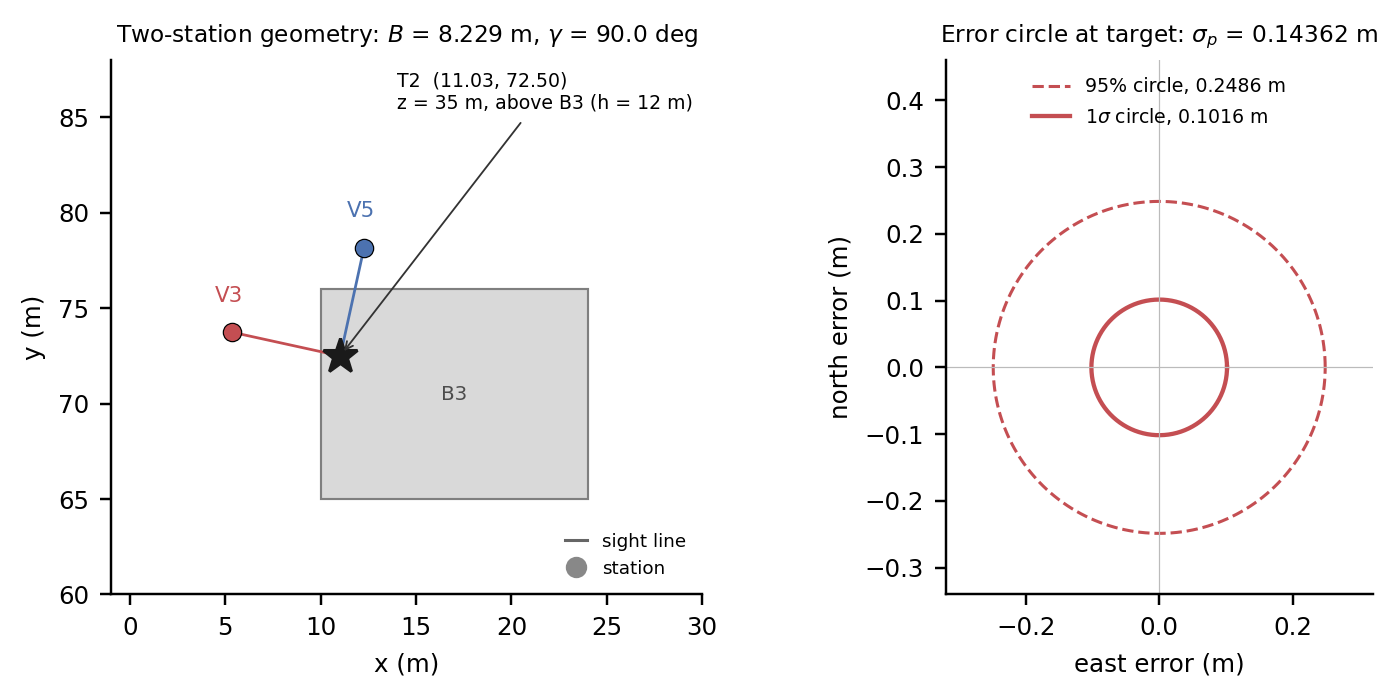
\includegraphics[width=0.95\textwidth]{fig7_q21.png}
  \caption{Optimal two-station geometry for T2. Left: both stations sit on the $r=r_{\mathrm{lb}}$ circle around a target that flies above B3. Right: because $\gamma=90^\circ$ and $r_1=r_2$ the error ellipse degenerates to a circle, so a single radius characterises the accuracy.}
  \label{fig:q21}
\end{figure}

That $\sigma_p$ lands exactly on the closed-form bound is not a coincidence: the two constraints on $r$ and $\gamma$ can be activated simultaneously, and equal ranges are easy to achieve when the target sits near a corner of the block. The independent differential-evolution and Nelder--Mead runs\cite{storn1997,nelder1965} return the same value to four decimals, confirming the optimum is not a search artefact.

\subsection{Problem 2(2)}

Enumeration gives $t_{\mathrm{last}}=10.655$ s. The structure is: \textbf{V3 is reused}, serving T1 and then T3 \emph{from the same station} $(13.5,91.0)$; V5 partners T1, V1 partners T3, and T2 is served independently by V2 and V4 (Table~\ref{tab:q22}, Figure~\ref{fig:gantt}).

\begin{table}[htbp]
  \centering
  \caption{Optimal schedule for three concurrent alerts.}
  \label{tab:q22}
  \small
  \begin{tabular}{lcccccc}
    \toprule
    Alert & Start (s) & Vehicles & Stations (m) & $r$ (m) & Elev. (deg) & $\sigma_p$ (m) \\
    \midrule
    T1 & $\bm{2.678}$ & V3 & $(13.5,\ 91.0)$ & $74.18$ & $30.1$ & \multirow{2}{*}{$5.004$} \\
       &              & V5 & $(49.5,\ 93.5)$ & $42.28$ & $45.5$ & \\
    T2 & $\bm{10.255}$ & V2 & $(72.5,\ 1.5)$ & $93.91$ & $19.4$ & \multirow{2}{*}{$2.828$} \\
       &               & V4 & $(87.5,\ 71.5)$ & $76.48$ & $23.3$ & \\
    T3 & $\bm{10.655}$ & V3 & $(13.5,\ 91.0)$ & $90.47$ & $30.4$ & \multirow{2}{*}{$2.090$} \\
       &               & V1 & $(14.5,\ 14.5)$ & $45.35$ & $49.5$ & \\
    \midrule
    \multicolumn{7}{l}{\footnotesize Angles $17.33^\circ$, $48.37^\circ$, $57.67^\circ$ (all $\ge15^\circ$); objective $\max_j\tau_j=10.655$ s.}\\
    \bottomrule
  \end{tabular}
\end{table}

\begin{figure}[htbp]
  \centering
  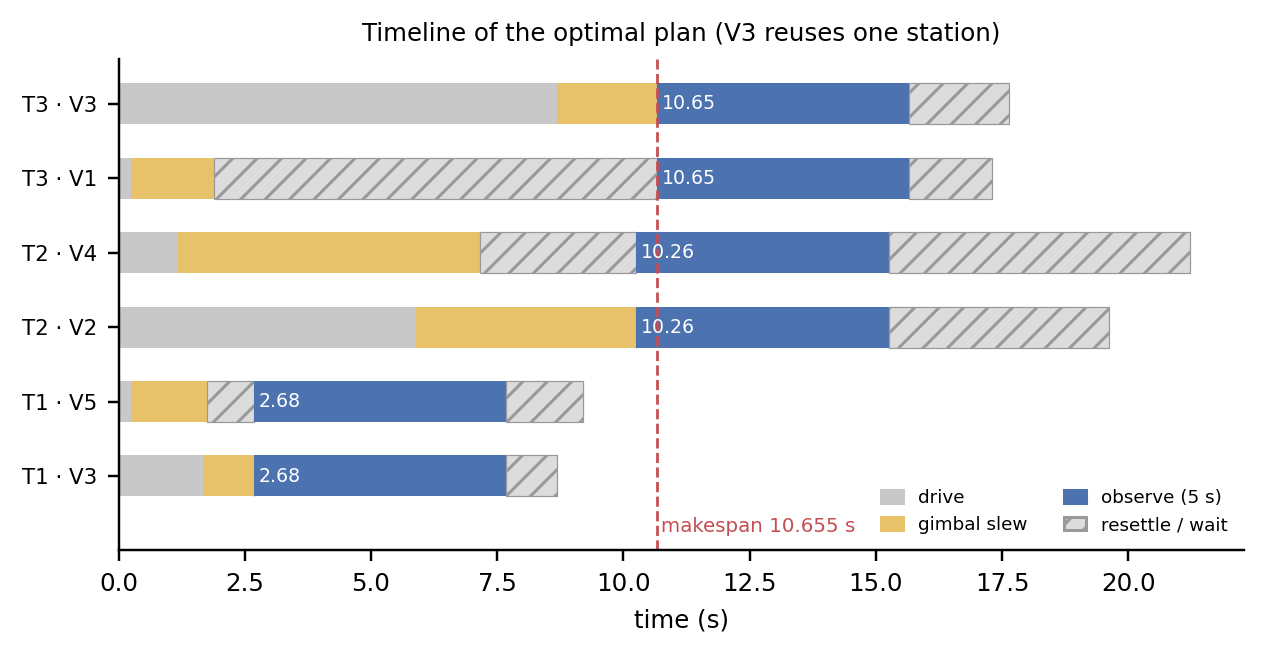
\includegraphics[width=0.95\textwidth]{fig4_gantt.png}
  \caption{Gantt chart of the optimal plan. V3's three phases (drive, observe T1, resettle, observe T3) follow back to back with no idle time; T3's start is the makespan.}
  \label{fig:gantt}
\end{figure}

The value decomposes exactly along the chain
\begin{equation}
\label{eq:chain}
t_{\mathrm{last}}=\tau^{\mathrm{T1}}_{\mathrm{start}}+5+t_{\mathrm{gim}}+t_{\mathrm{travel}}
=2.678+5+1.003+1.973=10.654\ \mathrm{s},
\end{equation}
one millisecond short of the simulated $10.655$ s. Here $1.003$ s is the slew from the T1 bearing to the T3 bearing (the longer of the azimuth and elevation axes), and $1.973$ s is the residual wait under same-station reuse---note that the ``travel'' is zero, and what remains is attitude adjustment.

Had reuse required repositioning, T3 would need a fresh station at least $30$ m away, i.e.\ $10$ s, pushing $t_{\mathrm{last}}$ past $20$ s. That is the entire value of the structural insight (Figure~\ref{fig:layout}).

\paperfig[0.66]{fig3_layout.png}{Station layout of the optimal plan. T1 and T3 are more than 90 m apart as targets, yet they share the station $(13.5,91.0)$, so V3's reuse requires no repositioning. T2 lies on the opposite side and shares almost no vehicle pool with T1/T3.}{fig:layout}

Against a nearest-assignment heuristic (no reuse), which gives $19.691$ s, the plan is $9.036$ s faster ($45.9\%$). The price is a slightly higher mean $\sigma_p$ ($3.307$ versus $2.933$ m), because time is the objective. Imposing an accuracy constraint instead ($\gamma\ge60^\circ$, $r\le45$ m) yields $16.843$ s with mean $\sigma_p=0.788$ m. These are two ends of a time--accuracy Pareto front (Table~\ref{tab:pareto}).

\begin{table}[htbp]
  \centering
  \caption{Time--accuracy trade-off across three configurations.}
  \label{tab:pareto}
  \begin{tabular}{lcccc}
    \toprule
    Configuration & $t_{\mathrm{last}}$ (s) & vs.\ best & mean $\sigma_p$ (m) & Note \\
    \midrule
    Nearest assignment (baseline) & $19.691$ & $+84.8\%$ & $2.933$ & no reuse \\
    This paper, $\gamma\ge15^\circ$ & $\bm{10.655}$ & -- & $3.307$ & same-station reuse \\
    Accuracy-first, $\gamma\ge60^\circ$, $r\le45$ m & $16.843$ & $+58.1\%$ & $\bm{0.788}$ & precision priority \\
    Degenerate control, $\gamma\ge0.5^\circ$ & $10.655$ & $0.0\%$ & $3.307$ & identical solution \\
    \bottomrule
  \end{tabular}
\end{table}

The last row is a deliberate negative test: relaxing the intersection gate from $15^\circ$ to $0.5^\circ$ changes nothing. The scenario in which time is sacrificed to satisfy an intersection angle simply never arises in this instance, so the result is insensitive to the exact value of the gate.

\subsection{Problem 3}

Equation \eqref{eq:smax} gives $s_{\max}=66.968$ m; the small-angle variant gives $66.922$ m, a $0.069\%$ gap that confirms first-order linearisation is adequate at this scale ($\sigma/r\le0.04$ rad).

\begin{table}[htbp]
  \centering
  \caption{Problem 3 results ($r=40$ m, gimbal $0.8^\circ/0.6^\circ$, tolerance $5^\circ$, confidence $95\%$).}
  \label{tab:q3}
  \small
  \begin{tabular}{lcc}
    \toprule
    Quantity & Exact ($\arctan$) & Small-angle \\
    \midrule
    Admissible $\sigma_{\Delta\psi}$ & \multicolumn{2}{c}{$2.55107^\circ$} \\
    Admissible position error & $1.63936$ m & $1.63845$ m \\
    Maximum travel $s_{\max}$ & $\bm{66.968}$ m & $66.922$ m \\
    \midrule
    At $s=0$: $\sigma_{\Delta\psi}$ / pass rate & $1.0884^\circ$ / $0.999996$ & -- \\
    At $s=80$: $\sigma_{\Delta\psi}$ / pass rate & $2.8975^\circ$ / $0.91558$ & -- \\
    Shortfall at $80$ m & \multicolumn{2}{c}{$0.3465^\circ$} \\
    \bottomrule
  \end{tabular}
\end{table}

At $80$ m the requirement \eqref{eq:constraint} reads $a+80b\le1.6394$ m. The nominal pair $(0.3,0.02)$ gives $1.90$ m, overshooting by $0.26$ m with a pass rate of only $0.9156$. The feasible triangle is $a\in[0,1.6394]$, $b\le(1.6394-a)/80$:
\begin{itemize}[leftmargin=2em]
  \item fixing $a=0.3$ requires $b\le0.016742$, i.e.\ $16.3\%$ below nominal;
  \item fixing $b=0.02$ requires $a\le0.0394$, an order of magnitude below nominal;
  \item with ideal ($a=0$) calibration, $b\le0.020492$, so the nominal $b$ would just pass.
\end{itemize}
The conclusion is sharp: at $80$ m the \emph{bias term} is the binding obstacle. Driving the bias near zero makes the nominal odometry coefficient acceptable, whereas improving $b$ alone while keeping $a=0.3$ cannot reach $0.95$ at any $b\ge0$.

Decomposing the variance (Figure~\ref{fig:q3sig}) locates an equal-contribution point at $s\approx19.91$ m: below it gimbal bias and control dominate, above it localisation dominates. At $s=66.97$ m the localisation term already accounts for $84.6\%$. The engineering priority therefore flips with range: calibrate the gimbal for short sorties, improve ranging for long ones.

\paperfig[0.95]{fig5_sigma.png}{Pointing-error propagation. Left: $\sigma_{\Delta\psi}$ against travelled distance with the $2.551^\circ$ criterion line; the crossing defines $s_{\max}=66.968$ m. Right: variance budget, showing gimbal errors dominating below the equal-contribution point $s\approx19.91$ m and localisation above it. At $s=80$ m the nominal model already fails, at a pass rate of $0.9156$.}{fig:q3sig}

\subsection{Problem 4}

We construct 93 scenarios: 36 new-alert cases (full grid over $\theta$ every $30^\circ$ and $R\in\{30,40,50\}$, because the observable region varies strongly with bearing), 5 vehicle-failure cases (all vehicles), 4 communication outages ($t_{\mathrm{rec}}=8,12,20,28$ s), and 48 stratified combinations. Table~\ref{tab:q4} compares keeping the plan (S0) with rescheduling (S1).

\begin{table}[htbp]
  \centering
  \caption{Comparison of S0 (keep) and S1 (reschedule) over 93 scenarios.}
  \label{tab:q4}
  \small
  \begin{tabular}{lcccccc}
    \toprule
    Category & $n$ & $\eta$: S0 $\to$ S1 & $t_{\mathrm{last}}$: S0 $\to$ S1 (s) & better & tie & worse \\
    \midrule
    New alert only & 36 & $1.000\to1.000$ & $25.033\to19.801$ & 36 & 0 & 0 \\
    Vehicle failure only & 5 & $0.733\to1.000$ & $10.847\to11.842$ & 4 & 1 & 0 \\
    Communication only & 4 & $1.000\to1.000$ & $27.236\to27.236$ & 0 & 4 & 0 \\
    Combined & 48 & $0.750\to1.000$ & $24.300\to24.995$ & 48 & 0 & 0 \\
    \midrule
    \textbf{All} & \textbf{93} & $\bm{0.857\to1.000}$ & $\bm{23.987\to22.374}$ & \textbf{88} & \textbf{5} & \textbf{0} \\
    \bottomrule
  \end{tabular}
\end{table}

The three disruption types buy different things, and this decomposition is the main practical finding.

\textbf{New alerts} already have $\eta=1$ (the original three alerts remain serviceable), so the entire gain is in \emph{time} ($-5.23$ s). Because reuse occupies only one vehicle, one vehicle is idle; the new alert is picked up immediately without preempting anything. In the typical case ($\theta=300^\circ$, $R=50$) the T4 start moves from $25.31$ s to $18.75$ s, a $6.57$ s improvement.

\textbf{Vehicle failures} raise $\eta$ from $0.733$ to $1.000$ at a cost of about $+1$ s. When a vehicle fails, its partner is left single-station and cannot intersect; another vehicle must be diverted from a closer position. The extra second is a \emph{necessary} sacrifice that buys $26.7$ percentage points of completeness.

\textbf{Communication outages} produce no difference at all. The outage only delays the command, and the remaining tasks of the original plan remain executable once it recovers. That a whole category yields zero change is itself evidence that the policy reacts to evidence rather than to the mere presence of a disruption.

\textbf{Combined cases} win on $\eta$ in all 48 instances ($0.75\to1.00$) for about $+0.70$ s, because a combined disruption typically removes both a vehicle and a slot at once---exactly the situation in which rescheduling is the only way back to a two-station fix.


\paperfig[0.72]{fig6_scenarios.png}{Per-scenario comparison of $t_{\mathrm{last}}$. Every point lies on or above the diagonal, so S1 never delays the makespan; hollow markers are the 52 scenarios in which completeness also improves.}{fig:q4sum}

% ============================================================
\section{Sensitivity and Validation}

\subsection{Five Independent Cross-Checks of the Shared Layer}

Because all sub-problems share one geometry engine, its correctness is a global precondition. We validate it with means that are independent of the main algorithms (Table~\ref{tab:valid}); all pass.

\begin{table}[htbp]
  \centering
  \caption{Independent cross-checks of the shared model layer.}
  \label{tab:valid}
  \footnotesize
  \begin{tabular}{clllc}
    \toprule
    ID & Object & Independent method & Result & Verdict \\
    \midrule
    V1 & Drivable set & 20\,000 points, brute force & 0 mismatches & pass \\
    V2 & Line of sight & 1\,800 pairs, per-face analytic & 0 mismatches & pass \\
    V3 & Shortest path & 0.005 m sampling for wall crossing & 0 crossings & pass \\
    V4 & Gimbal slew & 5 hand cases (wrap-around, unequal axes) & 5/5 match & pass \\
    V5 & Timeline & hand-computed arrive--observe--reset & matches & pass \\
    \bottomrule
  \end{tabular}
\end{table}

Check V3 deserves a note. Our first implementation compared grid A* with the visibility graph by path \emph{length} and obtained the paradoxical result that the grid was shorter. The cause was that the discrete grid smoothed away corners and let the path clip through a building. We therefore abandoned length comparison in favour of a direct \emph{wall-crossing audit}, which is the real feasibility criterion. After the fix, the visibility path has zero crossings at $0.005$ m sampling and is never longer than the grid path.

\subsection{Sensitivity}

Table~\ref{tab:sens1} varies the elevation cap for Problem 1. Tightening it from $80^\circ$ to $78^\circ$ costs $17.0\%$ of $Q$; to $70^\circ$, $51.6\%$. The optimum is therefore highly sensitive to a hardware specification---how high the gimbal can point. At $70^\circ$ the best station is no longer pressed against the boundary but retreats to $15.65$ m, and the feasible arc share also falls from $78.85\%$ to $64.58\%$, so siting options shrink as well.

\begin{table}[htbp]
  \centering
  \caption{Sensitivity of Problem 1 to the elevation cap.}
  \label{tab:sens1}
  \begin{tabular}{ccccc}
    \toprule
    Elevation cap & $r_{\mathrm{lb}}$ (m) & $Q$ ($\mathrm{m^{-1}}$) & Feasible arc share & $Q$ loss \\
    \midrule
    $80^\circ$ (nominal) & $7.5821$ & $0.131890$ & $78.85\%$ & -- \\
    $78^\circ$ & $9.1399$ & $0.109410$ & $78.08\%$ & $-17.0\%$ \\
    $75^\circ$ & $11.5218$ & $0.086792$ & $77.37\%$ & $-34.2\%$ \\
    $70^\circ$ & $15.6507$ & $0.063895$ & $64.58\%$ & $-51.6\%$ \\
    \bottomrule
  \end{tabular}
\end{table}

For Problem 2(1) the sensitivity is the $1/|\sin\gamma|$ factor of \eqref{eq:sigmap}: at a $20$ m range, $\sigma_p=0.494$ m at $\gamma=90^\circ$, $0.987$ m at $30^\circ$, $2.843$ m at $10^\circ$ and $28.286$ m at $1^\circ$. This is precisely why Problem 2(2) needs the $\gamma\ge15^\circ$ gate: below it, no amount of proximity rescues the accuracy.

For Problem 3, \eqref{eq:constraint} gives the marginal rate directly: with $b=0.02$, every $0.1$ m of bias costs $5$ m of operating radius.

\subsection{Monte Carlo and Statistical Checks}

Problem 2(1): 200\,000 samples give an empirical RMS of $0.14364$ m against the first-order $0.14362$ m, a $0.01\%$ deviation; the empirical $95\%$ quantile $0.24858$ m matches the analytic $0.2486$ m\cite{robert2004mc}.

Problem 3: two million samples give a maximum absolute deviation of $0.0069^\circ$ ($<0.3\%$). At $s_{\max}=66.968$ m the Monte Carlo pass rate is $0.94971$ against the analytic $0.95$, a $0.0003$ discrepancy that validates the inversion. Kolmogorov--Smirnov tests at $s=66.97$ and $s=80$ give $p=0.9168$ and $p=0.6651$, so normality is not rejected and using a normal quantile in \eqref{eq:crit} is legitimate.

Second-order check: comparing exact $\arctan$ with the linear approximation gives relative deviations of $0.2445\%$ at $s=20$ m and $0.12\%$ at $s=80$ m, so linearisation contributes at most a per-mille effect.

\subsection{Lower-Bound Audit}

Every sub-problem is compared against its own analytical bound (Table~\ref{tab:lower}). A result far above its bound signals a local optimum; a result below it signals an implementation error. This two-sided squeeze turned out to be the most effective correctness test we used.

\begin{table}[htbp]
  \centering
  \caption{Audit of each result against its analytical bound.}
  \label{tab:lower}
  \begin{tabular}{llll}
    \toprule
    Sub-problem & Bound & Computed & Gap \\
    \midrule
    Problem 1, $r$ & $7.58206$ m & $7.5821$ m & $+0.04$ mm \\
    Problem 2(1), $\sigma_p$ & $0.14362$ m & $0.14362$ m & $0.00$ \\
    Problem 2(2), $t_{\mathrm{last}}$ & $10.654$ s (hand chain) & $10.655$ s & $+1$ ms \\
    Problem 3, $s_{\max}$ & $66.968$ m, pass $0.95$ & MC $0.94971$ & $-0.0003$ \\
    Problem 4 & $(\eta,t_{\mathrm{last}})$ of S0 & S1 $\ge$ S0, 0 losses & -- \\
    \bottomrule
  \end{tabular}
\end{table}

% ============================================================
\section{Model Evaluation}

\subsection{Strengths}

\begin{enumerate}[leftmargin=2em]
  \item \textbf{Provable rather than merely numerical optima.} Problems 1 and 2(1) admit closed-form bounds whose attainability we verify, so the answers do not depend on grid resolution or random seeds and can be audited.
  \item \textbf{Single source of truth.} All five sub-problems share one geometry, occlusion and timeline implementation, eliminating the class of errors in which separately written geometries silently disagree; the layer is itself validated five ways.
  \item \textbf{Structural scheduling.} Recognising same-station reuse reduces Problem 2(2) from continuous-time optimisation to a 360-case enumeration, which is both globally optimal and fast enough ($85$ s) to be recomputed online.
  \item \textbf{Monotone rescheduling.} Equation~\eqref{eq:fallback} converts ``never worse'' from an expectation into a guarantee, and the experiment confirms zero losses in 93 scenarios.
\end{enumerate}

\subsection{Weaknesses and Future Work}

\begin{enumerate}[leftmargin=2em]
  \item \textbf{Station discretisation.} The candidate pools of Problem 2(2) bin azimuth at $5^\circ$, so $10.655$ s is optimal \emph{within that discretisation}; no gap bound to the continuous optimum is provided. A branch-and-bound wrapper or a continuous refinement from the current solution would close this.
  \item \textbf{Scenario set is not exhaustive.} The combined category of Problem 4 is a stratified sample. The $88/5/0$ result therefore holds statistically; rare adversarial combinations (failure plus long outage plus a distant new alert) may be under-represented.
  \item \textbf{Static target.} We assume the target is stationary during the $5$ s exposure. For a fast manoeuvring target the simultaneous-observation assumption still holds, but the intersection needs motion compensation; treating the in-window displacement as an extra unknown, estimable from a third station or a two-phase observe--reobserve scheme, is the natural extension.
  \item \textbf{First-order error model.} Linearisation error grows with $\sigma/r$; it is below $0.25\%$ here but would need second-order terms for a much larger operating area or much lower elevations.
  \item \textbf{No wind disturbance or communication jitter} on the measurements themselves; outages are modelled only as delayed triggers.
\end{enumerate}

\subsection{Generalisation}

The three-layer structure (geometry, measurement, decision) transfers directly to:
\begin{itemize}[leftmargin=2em]
  \item \textbf{Persistent multi-target surveillance}, replacing ``fastest single pass'' with a revisit-interval objective, which turns the reuse structure from ``one vehicle, two alerts'' into a vehicle routing problem with time windows.
  \item \textbf{Three-dimensional urban occlusion}, replacing closed boxes with arbitrary polyhedra or point clouds and the slab test with BVH-accelerated ray casting; the ``analytical bound plus arc enumeration'' idea survives, with the optimal set becoming a spherical patch.
  \item \textbf{Heterogeneous sensor networks}, where ranging radars and angle-only cameras coexist; the covariance \eqref{eq:cov} extends to a mixed observation matrix, and the bound follows from the trace of the inverse Fisher information.
\end{itemize}

% ============================================================
\section{Conclusion}

Within the stated constraints we established five results. (i) The single-station optimum is governed entirely by the elevation cap; it is analytically computable, globally attainable, and becomes unique under an explicit engineering tie-break, giving $r=7.5821$ m at $(88.8247,76.3233)$. (ii) The two-station intersection error is minimised when both ranges hit their lower bound and the intersection angle is $90^\circ$, giving $\sigma_p=0.14362$ m, exactly the closed-form bound. (iii) The three-alert scheduling problem is solved in $10.655$ s, and its structure is not a routing trick but a geometric coincidence: one vehicle can serve two alerts from a single station, eliminating repositioning altogether. (iv) At $80$ m the pointing requirement fails for the nominal error model, and the binding term is the bias, not the range coefficient---a conclusion with a clear procurement implication. (v) Under disruption, rescheduling never loses and its value is mainly completeness, not speed.

The recurring methodological lesson is that a bound is worth more than a search: it certifies optimality, resolves ties reproducibly, and exposes which physical parameter actually controls the answer.

% ============================================================
\begin{thebibliography}{99}
\small

\bibitem{torrieri1984}
Torrieri, D. (1984). Statistical theory of passive location systems. \emph{IEEE Transactions on Aerospace and Electronic Systems}, AES-20(2), 183--198. doi:10.1109/TAES.1984.310439

\bibitem{dijkstra1959}
Dijkstra, E. W. (1959). A note on two problems in connexion with graphs. \emph{Numerische Mathematik}, 1(1), 269--271. doi:10.1007/BF01386390

\bibitem{lozano1979}
Lozano-P\'erez, T., \& Wesley, M. A. (1979). An algorithm for planning collision-free paths among polyhedral obstacles. \emph{Communications of the ACM}, 22(10), 560--570. doi:10.1145/359156.359164

\bibitem{storn1997}
Storn, R., \& Price, K. (1997). Differential evolution---a simple and efficient heuristic for global optimization over continuous spaces. \emph{Journal of Global Optimization}, 11(4), 341--359. doi:10.1023/A:1008202821328

\bibitem{nelder1965}
Nelder, J. A., \& Mead, R. (1965). A simplex method for function minimization. \emph{The Computer Journal}, 7(4), 308--313. doi:10.1093/comjnl/7.4.308

\bibitem{hepner1987}
Hepner, S., \& Geering, H. (1987). On the observability of target maneuvers via bearing-only and bearing-rate-only measurements. In \emph{Proceedings of the AIAA Guidance, Navigation and Control Conference}. doi:10.2514/6.1987-2382

\bibitem{he2015aoa}
He, Y., Behnad, A., \& Wang, X. (2015). Accuracy analysis of the two-reference-node angle-of-arrival localization system. \emph{IEEE Wireless Communications Letters}, 4(3), 329--332. doi:10.1109/LWC.2015.2415788

\bibitem{qu2013coop}
Qu, Y., Wu, J., \& Zhang, Y. (2013). Cooperative localization based on the azimuth angles among multiple UAVs. In \emph{2013 International Conference on Unmanned Aircraft Systems (ICUAS)}, 818--823. doi:10.1109/ICUAS.2013.6564765

\bibitem{kumar2009ptz}
Kumar, P., Dick, A., \& Sheng, T. S. (2009). Real time target tracking with pan tilt zoom camera. In \emph{2009 Digital Image Computing: Techniques and Applications}, 492--497. doi:10.1109/DICTA.2009.84

\bibitem{robert2004mc}
Robert, C. P., \& Casella, G. (2004). \emph{Monte Carlo Statistical Methods} (2nd ed.). New York: Springer. doi:10.1007/978-1-4757-4145-2

\bibitem{kapoor1988vis}
Kapoor, S., \& Maheshwari, S. N. (1988). Efficient algorithms for Euclidean shortest path and visibility problems with polygonal obstacles. In \emph{Proceedings of the Fourth Annual Symposium on Computational Geometry (SCG '88)}, 172--182. doi:10.1145/73393.73411

\bibitem{sasiadek2008vision}
Sasiadek, J., \& Walker, M. (2008). Vision-based UAV navigation. In \emph{AIAA Guidance, Navigation and Control Conference and Exhibit}. doi:10.2514/6.2008-6667

\end{thebibliography}

% ============================================================
\newpage
\appendix
\section{Supporting Material}
\sloppy
\begin{enumerate}[leftmargin=2em]
  \item Paper source: \texttt{main.tex} (compiled with pdf\LaTeX).
  \item Shared model layer: \texttt{common/model.py} (geometry, occlusion, gimbal, shortest path, timeline) and \texttt{common/planner.py} (candidate pools, structural enumeration).
  \item Per-problem solver directories \texttt{Q1*/code}, \texttt{Q2-1*/code}, \texttt{Q2-2*/code}, \texttt{Q3*/code}, \texttt{Q4*/code}.
  \item Results: one \texttt{output} folder of JSON/CSV files per problem, plus a consolidated \texttt{summary.json}.
  \item Figures: PNG sources for both language versions, under the paper folder.
  \item Validation report: \texttt{model\_validation.json}.
\end{enumerate}

\section{Core Code}

\noindent\textbf{B.1 Line-of-sight test (slab method, vectorised)}
\begin{lstlisting}
def los_blocked(p, target, rects):
    """True if segment p->target hits any closed axis-aligned box."""
    p = np.asarray(p, float); q = np.asarray(target, float)
    d = q - p
    d_safe = np.where(np.abs(d) < 1e-12, 1e-12, d)
    tmin = (rects[:, 0:3] - p) / d_safe      # (n,3)
    tmax = (rects[:, 3:6] - p) / d_safe
    lo = np.minimum(tmin, tmax)
    hi = np.maximum(tmin, tmax)
    inside = np.abs(d) < 1e-12               # degenerate axis
    lo = np.where(inside, -np.inf, lo)
    hi = np.where(inside, np.inf, hi)
    t_enter = lo.max(axis=1)
    t_exit = hi.min(axis=1)
    hit = (t_enter <= t_exit) & (t_enter <= 1.0) & (t_exit >= 0.0)
    return bool(hit.any())
\end{lstlisting}

\noindent\textbf{B.2 Two-station accuracy and its closed-form bound}
\begin{lstlisting}
def sigma_p(s1, s2, target, sigma_deg=1.0):
    """RMS position error of two-station bearing intersection (meters)."""
    r1 = np.hypot(*(np.asarray(s1) - target[:2]))
    r2 = np.hypot(*(np.asarray(s2) - target[:2]))
    a1 = np.arctan2(target[1] - s1[1], target[0] - s1[0])
    a2 = np.arctan2(target[1] - s2[1], target[0] - s2[0])
    gamma = abs(np.degrees(np.arctan2(np.sin(a1 - a2), np.cos(a1 - a2))))
    s = np.radians(sigma_deg)
    return s * np.sqrt(r1**2 + r2**2) / abs(np.sin(np.radians(gamma)))

def sigma_p_lower_bound(H, h_cam=2.0, el_max=80.0, sigma_deg=1.0):
    """Closed-form global lower bound: sigma * sqrt(2) * (H-h)/tan(el_max)."""
    r_lb = (H - h_cam) / np.tan(np.radians(el_max))
    return np.radians(sigma_deg) * np.sqrt(2.0) * r_lb, r_lb
\end{lstlisting}

\noindent\textbf{B.3 Structural enumeration with timeline evaluation (pseudocode)}
\begin{lstlisting}
best = (inf, None)
for pair in combinations(ALERTS, 2):            # reuse this alert pair
    for order in permutations(pair, 2):         # which is served first
        for v in VEHICLES:                      # the reused vehicle
            for partners in combinations(V - {v}, 2):
                for indep in combinations(V - {v} - partners, 2):
                    assign = build(pair, order, v, partners, indep)
                    stations = pick_stations(assign, gamma_min=15)
                    if stations is None:
                        continue
                    t = timeline(assign, stations)    # Eq. (5), forward pass
                    if t.last < best[0]:
                        best = (t.last, (assign, stations))
\end{lstlisting}

\end{document}
